\section{Drawing Graphs with Circular Arcs}
\label{sect:drawing-graphs-with-circular-arcs}

\begin{frame}
  \frametitle{Agenda}
  \begin{itemize}
    \item \light{\nameref{sect:introduction}}
    \item \light{\nameref{sect:minimizing-potential-energy}}
    \item \nameref{sect:drawing-graphs-with-circular-arcs} \begin{itemize}
      \item \nameref{subsect:application-definitions}
      \item \nameref{subsect:application-existence-of-drawings}
      \item \nameref{subsect:application-graph-decomposition}
      \item \nameref{subsect:application-generalized-coordinates}
      \item \nameref{subsect:application-potential-energy}
      \item \nameref{subsect:application-results}
      \item \nameref{subsect:application-demo}
    \end{itemize}
  \end{itemize}
\end{frame}

\subsection{Definitions}
\label{subsect:application-definitions}

\begin{frame}
  \frametitle{\insertsubsection}
  \begin{itemize}
    \item Drawing of ${G}$ with circular arcs \begin{itemize}
      \item Every edge ${e \in E}$ drawn as a circular arc ${\Gamma_e}$
      \item No vertices coincide
      \item No edges overlap
      \item No edge intersects any vertices other than its endpoints
    \end{itemize}
  \end{itemize}
  \centering
  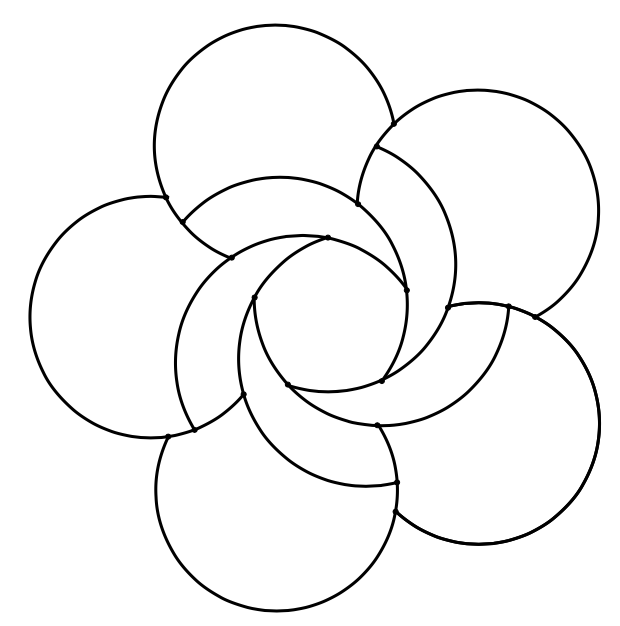
\includegraphics[height=3.5cm,natwidth=620,natheight=626]{Resources/Schulz.png}
\end{frame}

\begin{frame}
  \frametitle{\insertsubsection}
  \begin{itemize}
    \item Given a set ${\Pi = \lbrace P_1, \ldots, P_k \rbrace}$ of edge-disjoint paths \begin{itemize}
      \item ${V(\Pi) \coloneqq V(P_1) \cup \ldots \cup V(P_k)}$
      \item ${E(\Pi) \coloneqq E(P_1) \cupplus \ldots \cupplus E(P_k)}$
    \end{itemize}
    \item Drawing of ${\Pi}$ with circular arcs \begin{itemize}
      \item Drawing of ${G \coloneqq (V(\Pi), E(\Pi))}$ with circular arcs
      \item Each path ${P \in \Pi}$ is drawn as a circular arc ${\Gamma_P}$
    \end{itemize}
  \end{itemize}
  \centering
  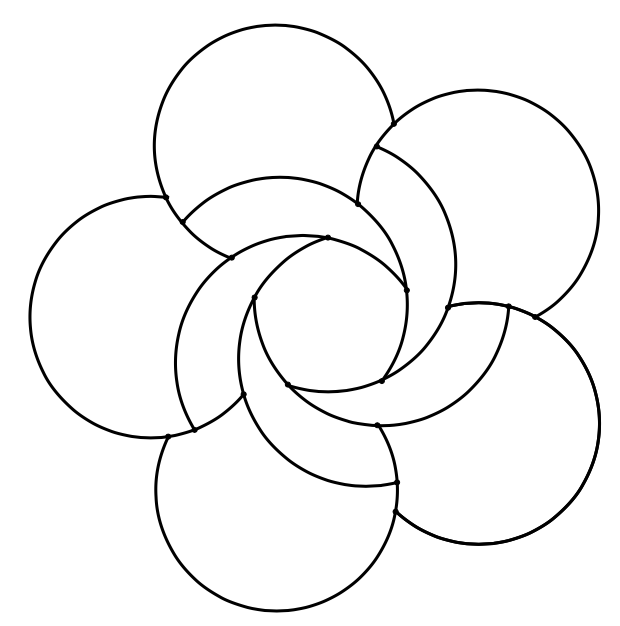
\includegraphics[height=3.5cm,natwidth=620,natheight=626]{Resources/Schulz.png}
\end{frame}

\subsection{Existence of Drawings}
\label{subsect:application-existence-of-drawings}

\begin{frame}
  \frametitle{\insertsubsection}
  \begin{itemize}
    \item Circles are determined by three distinct points
    \item Necessary condition: ${\abs{V(P_i) \cap V(P_j)} \leq 2 \quad \forall i \neq j}$ \begin{itemize}
      \item Condition is not sufficient!
    \end{itemize}
  \end{itemize}
  \begin{figure}
    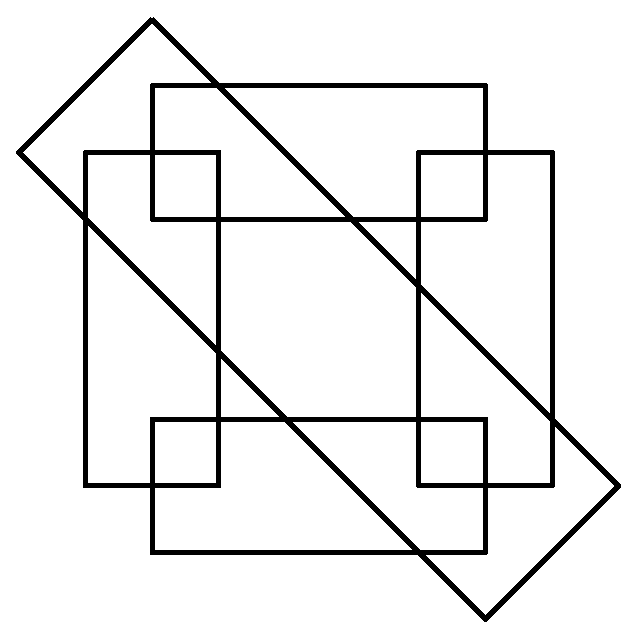
\includegraphics[height=3cm]{Resources/Arrangement-of-Pseudocircles}
    \quad
    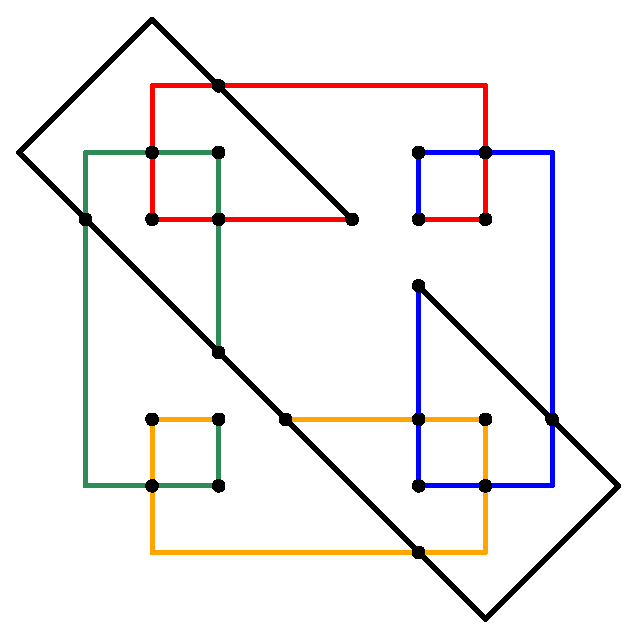
\includegraphics[height=3cm]{Resources/Arrangement-of-Pseudoarcs}
    \caption{An arrangement of pseudocircles that is not circleable (left) and a derived arrangement of pseudo circular arcs (right).}
  \end{figure}
\end{frame}

\begin{frame}
  \frametitle{\insertsubsection}
  \begin{itemize}
    \item Greedily realizable sequence of paths ${\Pi}$ \begin{itemize}
      \item Ordered sequence of edge-disjoint paths ${\Pi = (P_1, \ldots, P_k)}$
      \item ${V_\text{int}(P_i) \cap V(P_1 \cup \ldots \cup P_{i-1}) \stackrel{}{=} \varnothing, \quad i = 2 \ldots k}$
      \item Permits drawing with circular arcs using greedy algorithm
    \end{itemize}
  \end{itemize}
\end{frame}

\begin{frame}
  \frametitle{\insertsubsection}
  \begin{itemize}
    \item Greedily realizable sequence of paths ${\Pi}$ \begin{itemize}
      \item Ordered sequence of edge-disjoint paths ${\Pi = (P_1, \ldots, P_k)}$
      \item ${V_\text{int}(P_i) \cap V(P_1 \cup \ldots \cup P_{i-1}) \stackrel{}{=} \varnothing, \quad i = 2 \ldots k}$
      \item Permits drawing with circular arcs using greedy algorithm
    \end{itemize}
  \end{itemize}
  \begin{figure}
    \includegraphics<1>[height=4cm]{Resources/GreedyRealization-01}
    \includegraphics<2>[height=4cm]{Resources/GreedyRealization-02}
    \includegraphics<3>[height=4cm]{Resources/GreedyRealization-03}
    \includegraphics<4>[height=4cm]{Resources/GreedyRealization-04}
    \includegraphics<5>[height=4cm]{Resources/GreedyRealization-05}
    \includegraphics<6>[height=4cm]{Resources/GreedyRealization-06}
    \includegraphics<7>[height=4cm]{Resources/GreedyRealization-07}
    \includegraphics<8>[height=4cm]{Resources/GreedyRealization-08}
    \includegraphics<9>[height=4cm]{Resources/GreedyRealization-09}
    \includegraphics<10>[height=4cm]{Resources/GreedyRealization-10}
    \includegraphics<11>[height=4cm]{Resources/GreedyRealization-11}
    \caption{Greedy drawing of ${\Pi = ( \textit{abcde}, \textit{bfghd}, \textit{gijkl}, \textit{jmc} )}$}
  \end{figure}
\end{frame}

\begin{frame}
  \frametitle{\insertsubsection}
  \begin{itemize}
    \item Greedily realizable sequence of paths ${\Pi}$ \begin{itemize}
      \item Ordered sequence of edge-disjoint paths ${\Pi = (P_1, \ldots, P_k)}$
      \item ${V_\text{int}(P_i) \cap V(P_1 \cup \ldots \cup P_{i-1}) \stackrel{}{=} \varnothing, \quad i = 2 \ldots k}$
      \item Permits drawing with circular arcs using greedy algorithm
    \end{itemize}
    \item Characterization of vertices with respect to ${\Pi}$ \begin{itemize}
      \item Constrained vertices ${V_\text{c}(\Pi)}$: first appear as a path's internal vertex
      \item Unconstrained vertices ${V_\text{u}(\Pi)}$: first appear as a path's endpoint
    \end{itemize}
  \end{itemize}
\end{frame}

\subsection{Graph Decomposition}
\label{subsect:application-graph-decomposition}

\begin{frame}
  \frametitle{\insertsubsection}
  \begin{itemize}
    \item Find decomposition into greedily realizable sequence of (simple) paths
    \item Trivial decomposition ${\Pi = E}$ valid
    \item Non-trivial (greedy) graph decomposition \begin{itemize}
      \item Idea: append edges to working path until current head has been used before
    \end{itemize}
  \end{itemize}
  \centering
  \includegraphics<1>[height=4cm]{Resources/Graph-Decomposition-00.eps}
  \includegraphics<2>[height=4cm]{Resources/Graph-Decomposition-01.eps}
  \includegraphics<3>[height=4cm]{Resources/Graph-Decomposition-02.eps}
  \includegraphics<4>[height=4cm]{Resources/Graph-Decomposition-03.eps}
  \includegraphics<5>[height=4cm]{Resources/Graph-Decomposition-04.eps}
  \includegraphics<6>[height=4cm]{Resources/Graph-Decomposition-05.eps}
  \includegraphics<7>[height=4cm]{Resources/Graph-Decomposition-06.eps}
  \includegraphics<8>[height=4cm]{Resources/Graph-Decomposition-07.eps}
  \includegraphics<9>[height=4cm]{Resources/Graph-Decomposition-08.eps}
  \includegraphics<10>[height=4cm]{Resources/Graph-Decomposition-09.eps}
  \includegraphics<11>[height=4cm]{Resources/Graph-Decomposition-10.eps}
  \includegraphics<12>[height=4cm]{Resources/Graph-Decomposition-11.eps}
\end{frame}

\subsection{Generalized Coordinates}
\label{subsect:application-generalized-coordinates}

\begin{frame}
  \frametitle{\insertsubsection}
  \begin{itemize}
    \item Generalized coordinates \begin{itemize}
      \item \makebox[.5cm]{\hfill$x \colon$}\makebox[.9cm]{\hfill$V_\text{u}(\Pi)$} ${\to \mathbb{R}}$
      \item \makebox[.5cm]{\hfill$y \colon$}\makebox[.9cm]{\hfill$V_\text{u}(\Pi)$} ${\to \mathbb{R}}$
      \item \makebox[.5cm]{\hfill$\varphi \colon$}\makebox[.9cm]{\hfill$\Pi\phantom{)}$} ${\to (-180 \degrees, 180 \degrees)}$
      \item \makebox[.5cm]{\hfill$p \colon$}\makebox[.9cm]{\hfill$V_\text{c}(\Pi)$} ${\to (0, 1)}$
    \end{itemize}
  \end{itemize}
  \begin{figure}
    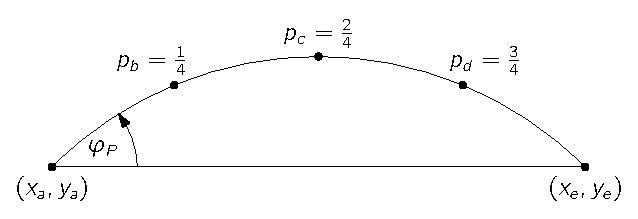
\includegraphics[height=2.0cm]{Resources/Generalized-Coordinates-Example.eps}
    \caption{Generalized coordinates for a single path ${P = abcde}$ with equi-length edges.}
  \end{figure}
\end{frame}

\begin{frame}[c]
  \frametitle{\insertsubsection}
  \begin{algorithm}[H]
    \caption{Transformation to Cartesian coordinates ${\vec{r}(v)}$}
    \SetKwData{CircularArc}{CircularArc}
    \SetKwData{PointForProgress}{pointForProgress}
    \ForEach{${v \in V_\text{u}(\Pi)}$}{
      ${\vec{r}(v) \gets (x({v}), y({v}))}$\;
    }
    \;
    \ForEach{${P = (v_1, \ldots, v_n) \in \Pi}$}{
      ${\Gamma(P) \gets \CircularArc(\vec{r}(v_1), \vec{r}(v_n), \varphi(P))}$\;
      \;
      \ForEach{${v \in (v_2, \ldots, v_{n-1})}$}{
        ${\vec{r}(v) \gets \Gamma(P).\PointForProgress(p(v))}$\;
      }
    }
    \;
  \end{algorithm}
\end{frame}

\subsection{Potential Energy}
\label{subsect:application-potential-energy}

\begin{frame}
  \frametitle{\insertsubsection}
  \begin{itemize}
    \item Vertex-Vertex repulsion \begin{itemize}
      \item Repulsive force based on Coulomb's law
      \item ${F_\text{rep}(d) \coloneqq c_1 \cdot \frac{1}{d^2}}$
    \end{itemize}
  \end{itemize}
  \begin{equation*}
    U_\text{rep}(u, v) \coloneqq{} \int\limits_{\infty}^{\mathclap{d(u, v)}} -F_\text{rep}(s) \differential{s}
  \end{equation*}
  \begin{itemize}
    \item Vertex-Vertex attraction \begin{itemize}
      \item Attractive force based on logarithmic spring
      \item ${F_\text{att}(l) \coloneqq -c_2 \cdot k \cdot \eval{\ln}{\frac{l}{k}}}$
    \end{itemize}
  \end{itemize}
  \begin{equation*}
    U_\text{att}(e) \coloneqq{} \int\limits_{k}^{\mathclap{l(\Gamma_e)}} -F_\text{att}(s) \differential{s}
  \end{equation*}
\end{frame}

\begin{frame}
  \frametitle{\insertsubsection}
  \begin{itemize}
    \item Order of vertices on a path \begin{itemize}
      \item Prevents intra-path overlapping edges
    \end{itemize}
  \end{itemize}
  \begin{equation*}
    U_\text{ord}(P) \coloneqq \begin{cases}
      0 & \text{if edges ${e \in E(P)}$ do not overlap} \\
      \infty & \text{otherwise}
    \end{cases} \hspace{0.25cm}
  \end{equation*}
  \begin{itemize}
    \item Vertex-Path repulsion \begin{itemize}
      \item Prevents unwanted vertex-edge intersections
      \item Prevents inter-path overlapping edges
    \end{itemize}
  \end{itemize}
  \begin{equation*}
    U_\text{int}(v, P) \coloneqq \begin{cases}
      c_3 \cdot \frac{1}{d(v, \Gamma_P)} & \text{if}~d(v, \Gamma_P) \neq 0 \\
      \infty & \text{otherwise}
    \end{cases}
  \end{equation*}
\end{frame}


\begin{frame}
  \frametitle{\insertsubsection}
  \begin{equation*}
  U \coloneqq
  \sum_{\mathclap{\substack{\lbrace u, v \rbrace \in V^2}}} U_\text{rep}(u, v)
  +
  \sum_{\mathclap{\substack{e \in E}}} U_\text{att}(e)
  +
  \sum_{\mathclap{\substack{P \in \Pi}}} U_\text{ord}(P)
  +
  \sum_{\mathclap{\substack{v \in V, P \in \Pi \\ v \notin V(P)}}} U_\text{int}(v, P)
  \end{equation*}
  \begin{itemize}
    \item Can be evaluated in ${\bigOh{\abs{V}^2 + \abs{E} + \abs{V} \cdot \abs{\Pi}}}$
    \item Optimization using hill climbing
  \end{itemize}
\end{frame}

\subsection{Results}
\label{subsect:application-results}

\newcommand{\drawing}[3]{\setlength\fboxsep{0pt}\colorbox{gray!10}{\makebox(75,75){\includegraphics[width=75pt,height=75pt,natwidth=#2,natheight=#3,keepaspectratio]{#1}}}}

\begin{frame}
  \frametitle{\insertsubsection}
  \begin{figure}
    \centerline{
      \drawing{Resources/Graph-10-09-1.pdf}{369}{291}\hspace{4pt}%
      \drawing{Resources/Graph-10-15-1.pdf}{267}{320}\hspace{4pt}%
      \drawing{Resources/Graph-10-20-1.pdf}{191}{145}\hspace{4pt}%
      \drawing{Resources/Graph-10-25-1.pdf}{122}{151}%
    }
    \vspace{3pt}
    \centerline{
      \drawing{Resources/Graph-10-09-2.pdf}{443}{196}\hspace{4pt}%
      \drawing{Resources/Graph-10-15-2.pdf}{253}{287}\hspace{4pt}%
      \drawing{Resources/Graph-10-20-2.pdf}{203}{165}\hspace{4pt}%
      \drawing{Resources/Graph-10-25-2.pdf}{203}{129}%
    }
    \caption{Drawings of graphs with 10 vertices and 9/15/20/25 edges; each with (bottom) and without (top) user adjustments.}
  \end{figure}
\end{frame}

\begin{frame}
  \frametitle{\insertsubsection}
  \begin{figure}
    \centerline{
      \drawing{Resources/Graph-15-14-1.pdf}{356}{362}\hspace{4pt}%
      \drawing{Resources/Graph-15-20-1.pdf}{356}{278}\hspace{4pt}%
      \drawing{Resources/Graph-15-25-1.pdf}{311}{248}\hspace{4pt}%
      \drawing{Resources/Graph-15-35-1.pdf}{276}{232}%
    }
    \vspace{3pt}
    \centerline{
      \drawing{Resources/Graph-15-14-2.pdf}{564}{404}\hspace{4pt}%
      \drawing{Resources/Graph-15-20-2.pdf}{341}{362}\hspace{4pt}%
      \drawing{Resources/Graph-15-25-2.pdf}{306}{271}\hspace{4pt}%
      \drawing{Resources/Graph-15-35-2.pdf}{262}{288}%
    }
    \caption{Drawings of graphs with 15 vertices and 14/20/25/35 edges; each with (bottom) and without (top) user adjustments.}
  \end{figure}
\end{frame}

\subsection{Demo}
\label{subsect:application-demo}

\begin{frame}
  \frametitle{\insertsubsection}
  \begin{itemize}
    \item Implemented as a Mac OS Application
    \item Written in Swift 3.0
  \end{itemize}
\end{frame}

